\newpage
\subsection{The TCP Server}
\label{subsec:server} 

In this subsection, we aim to illustrate the overall development of the TCP server operating the \textit{Toygether system}. As already mentioned, the server needs to be designed in order to bridge together plush toys and android users because communication between clients will always pass by the server itself. The software is required to implement the TCP protocol as well as the previously defined guidelines for the communication protocol (see subsection \ref{subsec:communication}).

\begin{figure}[ht]
    \centering
    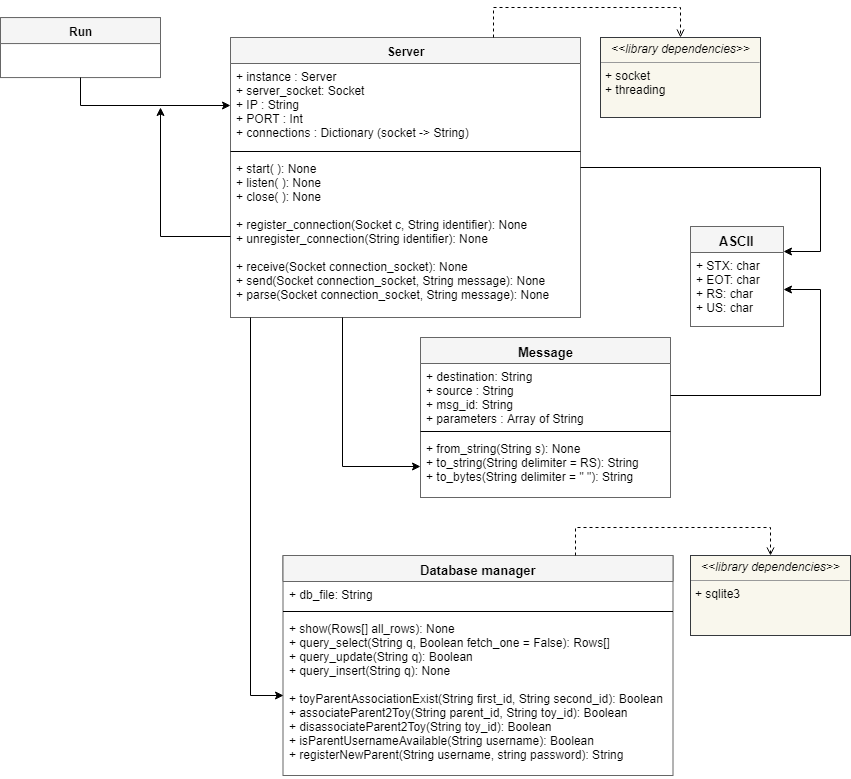
\includegraphics[scale=0.5]{images/SE_UML_server.png}
    \caption{UML class diagram for the Server software}
    \label{fig:SE_uml_server}
\end{figure}

Figure \ref{fig:SE_uml_server} illustrates, by adopting a UML class diagram, the overall structure of the server software. Thanks to numerous design choices, the complexity of the final architecture has been encapsulated in a relatively low number of constructing blocks. The aim of the upcoming pages will be to introduce each of the three main components of the structure (main server, message and database manager) in further detail, by reporting the reasoning on different implementation decisions encountered.

\newpage
Thanks to a stack diagram, illustrated in figure \ref{fig:SE_stack_server}, the reader can obtain an intuition regarding dependency levels between functions of the developed result. In particular, in order to implement the software, a choice of libraries has been made to obtain the base-code upon which the project could have been built on. Python standard libraries provide capable tools for our needs: firstly, the \textit{socket} library predisposes the necessary means to manage a TCP stream of incoming and outgoing communications with different clients; secondly, the \textit{sqlite3} library offers a collection of APIs to integrate SQL querying with an SQLite database. On top of such libraries, our components have been defined (see the next pages for further details).

\begin{figure}[ht]
    \centering
    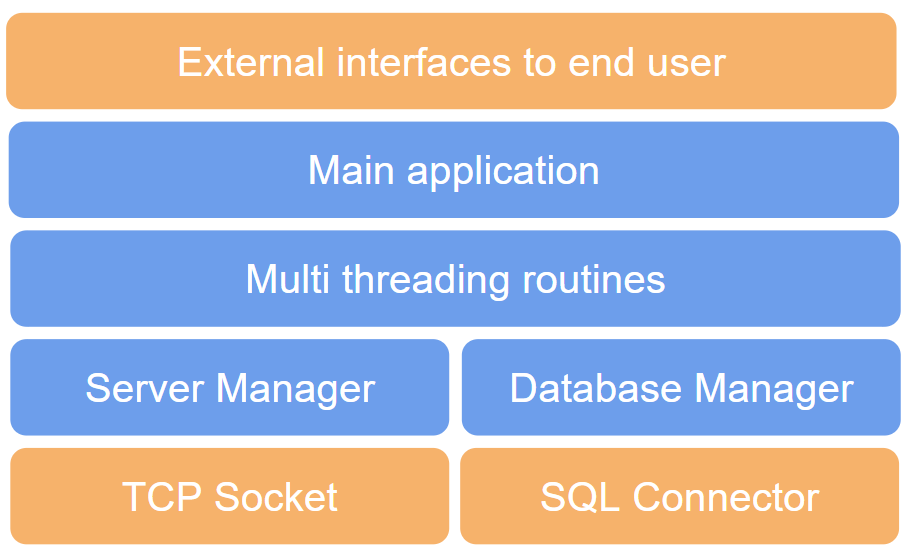
\includegraphics[scale=0.5]{images/SE_server_stack.PNG}
    \caption{Stack diagram for the Server software dependencies}
    \label{fig:SE_stack_server}
\end{figure}

\medskip
Before concluding this general introduction of the server software, a small extra detail in regards to the design choices needs to be appointed. Following guidelines in the book "\citetitle{gamma1995design}" by \textcite{gamma1995design} for well-construct software, the server application has been built as a so-called \textbf{Singleton}. This coding design prevents multiple instantiating procedures of the object within the same environment, which would be meaningless in our context. The software is, therefore, enriched with a class-method that transparently handles the design pattern implementation.

\vspace{0.5cm}
\lstinputlisting[style=Python]{code_snippets/python/server_singleton.py}
\vspace{0.5cm}
\lstinputlisting[style=Python]{code_snippets/python/server_singleton_use.py}
\vspace{0.5cm}

\newpage
\subsubsection{The main component: Server manager}
The fundamental operations managed by the server are handled by this main component. The objective of the following paragraphs will be to introduce the reader to all the methodologies applied in order to obtain a TCP server application, capable of handling the traffic of multiple connected clients. While developing the server, particular importance has been given to the design needs illustrated in the previous sections (parallel execution of clients, for example). In order to implement the component, the standard Python socket library has been studied and adopted for tasks of I/O stream management between server and clients.

\medskip
The component is executed by the \textit{start()} function call, which main lines of code are illustrated below. The reader should be aware that, in order to convey programming information without overheads in terms of clarity, parts of the excess code with respect to the basic logic itself (i.e. try-catch clauses, output printing, etc.) have not been reported. In order to obtain a complete overview, the final code can be referenced. The function's task is to initiate an incoming stream for clients which aim to connect to the server afterwards. To this intent, the component predisposes an open stream by binding it to a defined IP address and port, which will then used as the reference point by connecting clients. For the constructed prototype, the choice of such values has been trivial (IP address equal to 192.168.1.10 and port equal to 6789).

\vspace{0.5cm}
\lstinputlisting[style=Python]{code_snippets/python/server_start.py}
\vspace{0.5cm}

After the initialisation of the stream, the server starts the listening procedure which will wait for an incoming connection. The next code includes a simplified pipeline for such procedure to be accomplished by the server. Whenever a new connection is identified, the server instantiates a socket that will handle all future exchanges. In fact, the server is able to manage multiple clients by keeping track of a unique socket for each of them. Within a socket, the communication between a client and a server is handled via point-to-point methodologies which isolates them from the rest of the environment. Furthermore, in order to parallelize the execution of all socket related tasks by the server, each new incoming connection is assigned to a thread. The parallel programming design allows the software to continue accepting new connections, which as mentioned before halts the main thread until a client is reached, while fully operate with each client and their socket.

\medskip
Due to the parallel environment, the server works in, peculiar situations might occur. For instance, multiple clients might request a connection with the server at the same time while the latter has not yet instantiated a thread for the previous connection made. In such situation, a queue is built (in the prototype context with five clients in hold) to shunt the workload. Such queue is dependant on the running system and will be further examined in the future when scaled up solutions will be faced.

\vspace{0.5cm}
\lstinputlisting[style=Python]{code_snippets/python/server_listen.py}
\vspace{0.5cm}

Each client-thread main task is to provide a listener for incoming messages received by such connected client. The communication is managed with a stream of bytes that are recorded by the software until the intended message has been fully broadcast (i.e. the end of transmission marker EOT has been detected, as previously described in the subsection \ref{subsec:communication}). Messages, afterwards, are parsed to determine which possible event they might trigger on the server itself or whether they need to be forwarded to a different client if correctly constructed.

\vspace{0.5cm}
\lstinputlisting[style=Python]{code_snippets/python/server_receive.py}
\vspace{0.5cm}

Although both \textit{parse()} and \textit{send()} functions could be fully explored as well, their execution is trivial compared to the previously presented components. The former provides an inspection of the received message and conditionally execute tasks according to the MSG\_ID contained. The latter, on the other hand, employs the Python library tools to broadcast a string constructed message on the stream. Such operation is handled, as well, in a different threaded execution to avoid interruptions on the receiving task.

\newpage
\subsubsection{The Message component}
The message's structure, introduced during the previous discussion over the communication protocol (see subsection \ref{subsec:communication}), is particularly appropriate to be used in conjunction with the help of the component we are about to illustrate. In fact, the pragmatic definition of records and units that construct each message can be managed by a class, whose attributes are associated with the message's records themselves. For this intent, the message component of the server is built to store \textit{source}, \textit{destination}, \textit{message id} and \textit{parameters} of each new incoming/outgoing communication.

\medskip
Furthermore, the message component becomes extremely useful whenever messages are required to be parsed by the server. The following code, for instance, provides a class-method which allows instantiating of new components via string arguments. In the previous subsection, the \textit{receive()} function of the server would instantiate a message component by using such method: given a correct lecture of the byte-stream (interpreted as a string), the message component can be constructed which would eventually provide easy access to the contained records and parameters.

\vspace{0.5cm}
\lstinputlisting[style=Python]{code_snippets/python/server_message_from_string.py}
\vspace{0.5cm}
\lstinputlisting[style=Python]{code_snippets/python/server_message_from_string_use.py}

\newpage
\subsubsection{The Database Manager component}
The last building block of the server application is composed of a series of functions to manage interactions with the main database. This latter corresponds to the basic data structure needed to store non-volatile information about the system status. 

\begin{figure}[ht]
    \centering
    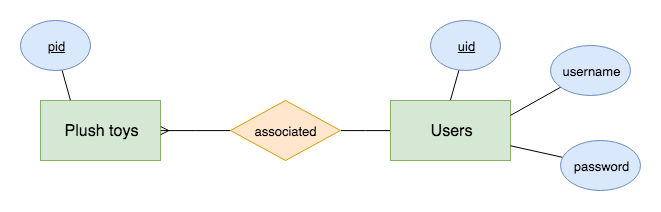
\includegraphics[scale=0.7]{images/SE_ERdiag.png}
    \caption{Entity relationship diagram for the database structure}
    \label{fig:SE_ERdiag}
\end{figure}

By adopting an Entity-Relationship diagram, Figure \ref{fig:SE_ERdiag} illustrates how the logical structure has been designed. The amount of information (at the present state) is not particularly big. However, it is crucial to store basic information about the system current state, by keeping track of registered users (to allow them sign-in privileges) and associated plush toy (once a pair of android app and toy have been paired together). This latter detail is of crucial importance for the server, as it covers the second advantage of the communication protocol designed (see section \ref{subsec:communication}). As already mentioned, the advantages of the communication protocol can be identified in both a higher abstraction and a message-forwarding filtering. Therefore, the Database Manager component can be used to consult the database itself, checking that SOURCE and DEST of the message are associated (paired) before forwarding to the destination. This operation filters incorrect or malicious messages, restricting communication to pairs of clients which have authorized the link.

\medskip
The following API has been implemented to correctly face database consultations by the server. Note that the reported list is only an intuition for the reader on the result obtained with this component. The communication with the database has been implemented via SQL and the provided python libraries for reaching the structure itself.

\vspace{0.5cm}
\lstinputlisting[style=Python]{code_snippets/python/server_database_API.py}